%% LyX 2.5.1 created this file.  For more info, see https://www.lyx.org/.
%% Do not edit unless you really know what you are doing.
\documentclass[brazil]{article}
\usepackage[T1]{fontenc}
\usepackage{textcomp}
\usepackage[utf8]{luainputenc}
\usepackage{colortbl}
\usepackage{url}
\usepackage{amsmath}
\usepackage{graphicx}
\usepackage{geometry}
\geometry{verbose,tmargin=3cm,bmargin=3cm,lmargin=3cm,rmargin=2.5cm}

\makeatletter

%%%%%%%%%%%%%%%%%%%%%%%%%%%%%% LyX specific LaTeX commands.
%% Because html converters don't know tabularnewline
\providecommand{\tabularnewline}{\\}

%%%%%%%%%%%%%%%%%%%%%%%%%%%%%% User specified LaTeX commands.







\makeatother

\usepackage{babel}
\begin{document}
\title{Resultados}
\maketitle

\section{Modelagem do circuito quântico}

Dado um vetor de entrada de dimensão $m$, o mesmo deve ser codificado usando $m$ coeficientes para definir uma função de onda geral $\left|\psi_{i}\right\rangle $. Na prática, dados vetores de entrada e pesos arbitrários temos: 
\begin{equation}
\overrightarrow{i}=\left(\begin{array}{c}
i_{0}\\
i_{1}\\
\vdots\\
i_{m-1}
\end{array}\right),\qquad\overrightarrow{w}=\left(\begin{array}{c}
w_{0}\\
w_{1}\\
\vdots\\
w_{m-1}
\end{array}\right).
\end{equation}
Dessa forma, pode-se definir os seguintes estados quânticos: 
\begin{equation}
\left|\psi_{i}\right\rangle =\frac{1}{\sqrt{m}}\sum^{m-1}_{j=0}i_{j}\left|j\right\rangle ,\qquad\left|\psi_{w}\right\rangle =\frac{1}{\sqrt{m}}\sum^{m-1}_{j=0}w_{j}\left|j\right\rangle .
\end{equation}
Os estados $\left|j\right\rangle =\in\left\{ \left|00\ldots00\right\rangle ,\left|00\ldots01\right\rangle ,\dots,\left|11\ldots11\right\rangle \right\} $ formam a base computacional do processador quântico, no qual vamos identificar cada estado por inteiros decimais que são formados a partir da respectiva string binária $\left|j\right\rangle \in\left\{ \left|0\right\rangle ,\left|1\right\rangle ,\dots,\left|m-1\right\rangle \right\} $. Evidentemente se há $N$ qubits no registrador, então haverá $m=2^{N}$ estados. Dessa maneira como motivação inicial, pode-se pensar em ter como objetivo que o circuito quântico seja capaz de efetuar o seguinte cálculo: 
\begin{equation}
\left\langle \psi_{i},\psi_{w}\right\rangle =\frac{\overrightarrow{w}\cdot\overrightarrow{v}}{m}.\label{prodin}
\end{equation}
Assumindo que os qubits são inicializados em $\left|00\dots00\right\rangle \equiv\left|0\right\rangle ^{\otimes N}$, o primeiro passo é preparar o estado $\left|\psi_{i}\right\rangle $ através de uma transformação unitária $U_{i}$ com os valores de entrada em $\overrightarrow{i}$ codificados. Ou seja, o operador de entrada deve ser capaz de realizar a seguinte transformação: 
\begin{equation}
U_{i}\left|0\right\rangle ^{\otimes N}=\left|\psi_{i}\right\rangle .
\end{equation}
Em princípio, qualquer matriz $m\times m$ unitária com $\overrightarrow{i}$ na primeira coluna serve. O próximo passo é realizar uma transformação unitária $U_{w}$ com os valores do peso $\overrightarrow{w}$ codificados de maneira que leve o resultado do produto interno da equação (\ref{prodin}) ao último coeficiente da base computacional. Explícitamente, queremos o seguinte comportamento: 
\begin{equation}
\begin{split}U_{w}\left|\psi_{i}\right\rangle  & =\left[\frac{1}{\sqrt{m}}\left(\begin{array}{cccc}
A_{11} & A_{21} & \cdots & A_{1\left(m-1\right)}\\
A_{12} & A_{22} & \cdots & A_{2\left(m-1\right)}\\
\vdots & \vdots & \ddots & \vdots\\
\overline{w_{0}} & \overline{w_{1}} & \ldots & \overline{w_{m-1}}
\end{array}\right)\right]\left[\left(\begin{array}{c}
i_{0}\\
i_{1}\\
\vdots\\
i_{m-1}
\end{array}\right)\frac{1}{\sqrt{m}}\right]\\
 & =\left(\begin{array}{c}
C_{1}\\
C_{2}\\
\vdots\\
\sum^{m-1}_{j=0}\overline{w_{j}}i_{j}
\end{array}\right)\frac{1}{m}.
\end{split}
\end{equation}
Onde $A_{ij}$ e $C_{i}$ denotam coeficientes irrelevantes para nosso propósito. Semelhante ao caso do operador de entrada, em princípio qualquer matriz $m\times m$ unitária com o conjugado de $\overrightarrow{w}$ na última linha serve. Porém, para justificar alguns algoritmos propostos nas próximas seções para construção do circuito mais algumas demonstrações matemáticas se tornam relevantes. Em especial, o operador $U_{w}$ deve ser capaz de realizar a seguinte transformação: 
\begin{equation}
U_{w}\left|\psi_{w}\right\rangle =\left|1\right\rangle ^{\otimes N}=\left|m-1\right\rangle .
\end{equation}
Onde $\left|m-1\right\rangle $ corresponde ao último estado da base computacional. Após a aplicação de ambos operadores, o estado final pode ser decomposto na base computacional, isto é: 
\begin{equation}
U_{w}U_{i}\left|0\right\rangle ^{\otimes N}=U_{w}\left|\psi_{i}\right\rangle =\sum^{m-1}_{j=0}c_{j}\left|j\right\rangle .
\end{equation}
Denotando o estado final como $\left|\phi_{i,w}\right\rangle \equiv U_{w}U_{i}\left|0\right\rangle ^{\otimes N}$ , e como $U_{w}$ é um operador unitário, então o produto interno entre $\left|\psi_{i}\right\rangle $ e $\left|\psi_{w}\right\rangle $ pode ser escrito como: 
\begin{equation}
\begin{split}\left\langle \psi_{w}|\psi_{i}\right\rangle  & =\left\langle \psi_{w}\left|U^{\dagger}_{w}U_{w}\right|\psi_{i}\right\rangle \\
 & =\left\langle m-1|\phi_{i,w}\right\rangle \\
 & =\sum^{m-1}_{j}c_{j}\left\langle m-1|j\right\rangle \\
 & =c_{m-1}.
\end{split}
\end{equation}
Torna-se evidente que o resultado que nos interessa é o coeficiente $c_{m-1}$ do estado final do processador após ambas transformações unitárias serem aplicadas. Ainda, podemos usar um qubit auxiliar $a$ inicialmente no estado $\left|0\right\rangle $ e um operador NOT multi-controlado entre os $N$ qubits que codificam a informação e o alvo $a$. Isto leva a: 
\begin{equation}
\left|\phi_{i,w}\right\rangle \left|0\right\rangle \rightarrow\sum^{m-2}_{j=0}c_{j}\left|j\right\rangle \left|0\right\rangle _{a}+c_{m-1}\left|m-1\right\rangle \left|1\right\rangle _{a}.
\end{equation}
Desse modo é necessário medir apenas a probabilidade do qubit auxiliar $a$ estar no estado $\left|1\right\rangle $. Concluindo, a saída final do circuito quântico que será medida é $\left|C_{m-1}\right|^{2}$. Então o valor a ser medido após a aplicação do algoritmo é: 
\begin{equation}
\left|\left\langle \psi_{w}|\psi_{i}\right\rangle \right|^{2}=\frac{\left|\overrightarrow{w}\cdot\overrightarrow{v}\right|^{2}}{m^{2}}.
\end{equation}
Um esquema geral do algoritmo responsável por este cálculo está ilustrado na figura \ref{UM}.

\begin{figure}[ht]
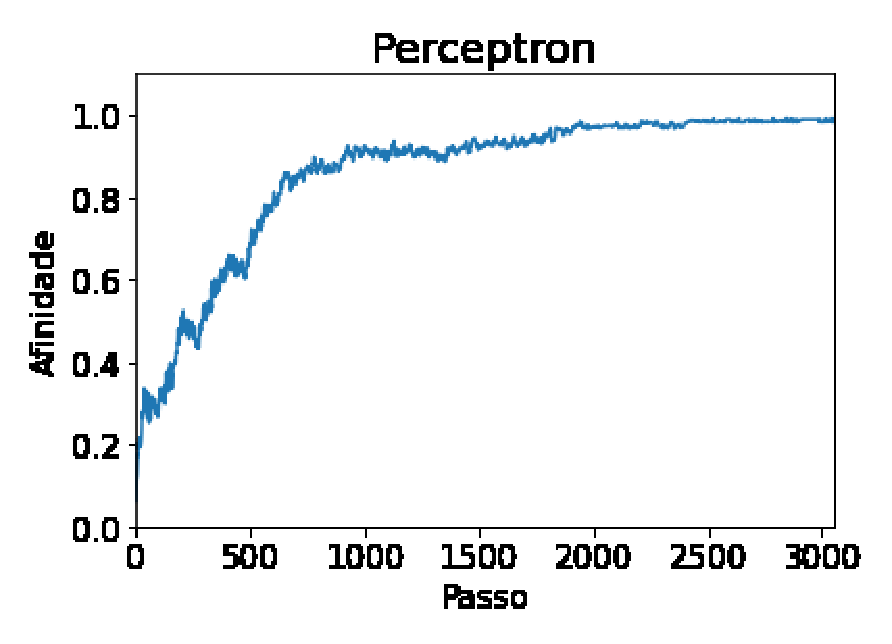
\includegraphics[width=0.75\textwidth]{img1} \centering \caption{Esquema geral do algoritmo quântico responsável pelo produto interno.}
\label{UM} 
\end{figure}


\section{Especificação das transformações unitárias}

O próximos dois algoritmos foram desenhados pensando nas redes neurais, isto é, trabalham apenas com a variação da fase dos números complexos. Em ambos os modelos, as variáveis de entradas e pesos estão presentes nas fases dos números complexos, isto é $i_{j},w_{j}\in\left\{ e^{i\theta}\right\} $, com $0\leq\theta\leq2\pi$, e a informação pode ser codificada em uma superposição uniforme de toda base computacional, já que alterar a fase do número complexo não altera seu módulo. Também podemos lembrar que o caso binário do perceptron se torna apenas um caso especial dos valores contínuos do sigmoide, para valores extremos de $\theta$.

\subsection{Bloco de rotação de fase }

Como primeira etapa, vamos definir um bloco de rotação de fase $B_{N,j}\left(\lambda\right)$ como uma transformação unitária atuando na base computacional de $N$ qubits da seguinte forma: 
\begin{equation}
B_{N,j}\left(\lambda\right)\left|j'\right\rangle =\left\{ \begin{array}{ccc}
e^{i\lambda}\left|j'\right\rangle  & ,\text{se} & j=j'\\
\left|j'\right\rangle  & ,\text{se} & j\neq j'
\end{array}\right..
\end{equation}
Podemos implementar uma família de blocos de rotação de fase para $N$ qubits usando uma rotação de fase multi-controlada $C_{u1}\left(\lambda\right)$ em combinação com operadores NOT em qubits unitários: 
\begin{equation}
B_{N,j}\left(\lambda\right)=O_{j}\left[C_{u1}\left(\lambda\right)\right]O_{j}.
\end{equation}
Onde $O_{j}=\otimes^{N}_{l=0}\left(NOT_{l}\right)^{1-j_{l}}$ é a expressão responsável por levar o coeficiente alvo para o estado $\left|m-1\right\rangle $ da base computacional. Então é possível aplicar a rotação de fase multi-controlada $C_{u1}\left(\lambda\right)$ tendo como alvo o qubit $N$. Desta maneira irá alterar a fase somente do coeficiente alvo, e então $O_{j}$ pode ser novamente utilizado para trazer o coeficiente a seu estado original. $NOT_{l}$ significa que aplicamos o operador $NOT$ no \textit{l-ésimo} qubit, e $j_{l}=0$ se o l-ésimo qubit está no estado $\left|0\right\rangle $ ($j_{l}=1$ se o estado for $\left|1\right\rangle $). É importante notar que $j_{l}=0$ implica em de fato aplicarmos a operação $NOT$ no qubit $l$, mas $j_{l}=1$ significa que usamos o operador identidade para manter o \textit{l-ésimo} qubit inalterado. Uma característica importante do bloco de rotação de fase é manter inalterado todos os coeficientes que não sejam o alvo.

Com o bloco de rotação de fase definido, pode-se resumir a sequência completa da implementação de $U_{i}$, lembrando da definição do operador de entrada ($U_{i}\left|0\right\rangle ^{\otimes N}=\left|\psi_{i}\right\rangle $) da seguinte forma: 
\begin{itemize}
\item Partindo do registrador inicializado em $\left|0\right\rangle ^{\otimes N}$, aplica-se operadores de Hadamard em cada qubit para criar um estado de total sobreposição entre todos os elementos da base computacional: $\left|0\right\rangle ^{\otimes N}\stackrel{H^{\otimes N}}{\rightarrow}\frac{1}{\sqrt{m}}\sum^{m-1}_{j=0}\left|j\right\rangle \equiv\left|\psi_{0}\right\rangle $; 
\end{itemize}
%
\begin{itemize}
\item Então é necessário apenas aplicar os blocos de rotação de fase nos coeficientes que forem necessários. 
\begin{itemize}
\item Como o bloco de rotação de fase mantém os outros coeficientes inalterados, deste modo a ordem de aplicação torna-se irrelevante. 
\end{itemize}
\end{itemize}
O operador $U_{w}$ é definido de maneira similar mas em ordem inversa. Levando em conta como é definido ($U_{w}\left|\psi_{w}\right\rangle =\left|1\right\rangle ^{\otimes N}=\left|m-1\right\rangle $), temos então: 
\begin{itemize}
\item Aplica-se os blocos de mudança de fase com negativo da fase do peso de forma que leve o estado computacional atual ao estado de sobreposição: $\left|\psi_{w}\right\rangle \stackrel{B_{N,j}\left(-\lambda\right)}{\rightarrow}\left|\psi_{0}\right\rangle $; 
\item Com o operador de Hadamard aplicado em cada qubit, o estado final do sistema se torna o estado inicial do processador, isto é: $\left|\psi_{0}\right\rangle \stackrel{H^{\otimes N}}{\rightarrow}\left|0\right\rangle ^{\otimes N}$; 
\item Então, com um operador NOT aplicado em cada qubit, o sistema vai para o estado desejado: $\left|0\right\rangle ^{\otimes N}\stackrel{NOT^{\otimes N}}{\rightarrow}\left|1\right\rangle ^{\otimes N}$. 
\end{itemize}
É interessante aqui destacar que o complexo conjugado de um número complexo qualquer $z=e^{i\lambda}$ equivale a outro número complexo de mesmo módulo e com uma fase equivalente ao seu negativo $\overline{z}=e^{-i\lambda}$. Portanto aplicar uma rotação de fase a $z$ equivalente ao negativo da sua própria fase equivale a multiplicar $z$ pelo seu conjugado: $\overline{z}z=e^{-i\lambda}e^{i\lambda}=1$. De forma que estamos construindo um operador $U_{w}$ que a última linha é o conjugado de $\overrightarrow{w}$, como desejamos.

\begin{figure}[ht]
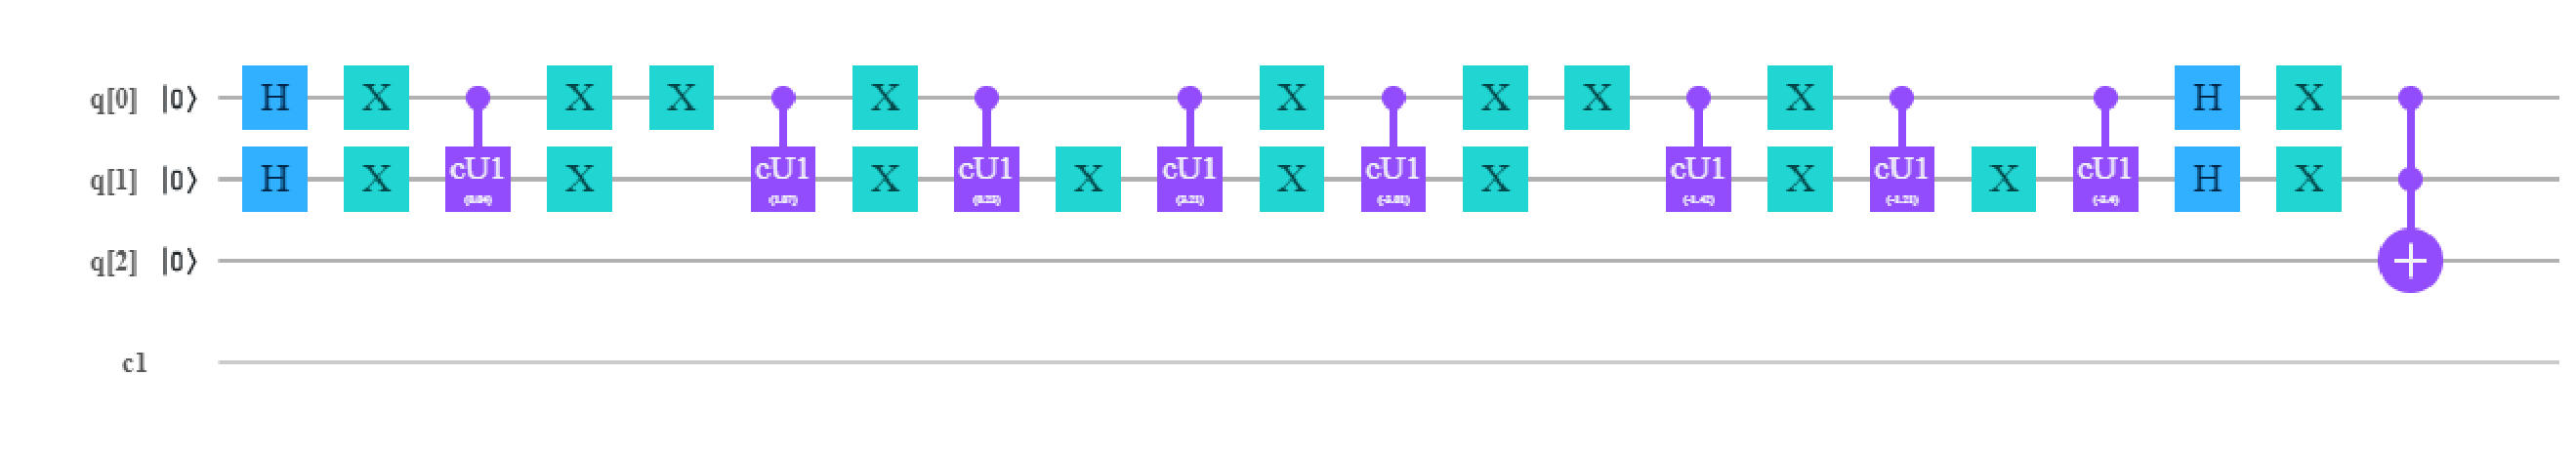
\includegraphics[width=1\textwidth]{img2} \centering \caption{Exemplo de circuito utilizando o algoritmo dos blocos de rotação de fase.}
\label{DOIS} 
\end{figure}

Um exemplo de circuito construído utilizando os blocos de rotação de fase está ilustrado na figura \ref{DOIS}.

\subsection{HSGS}

Uma solução que espera-se ser mais eficiente para variar a fase dos números complexos é o algoritmo HSGS. Este algoritmo espera-se ser capaz de reduzir os recursos quânticos necessários em comparação com o método dos blocos de rotação de fase apresentado anteriormente. Isto ocorre, principalmente, porque ainda que continue apresentando um custo exponencial, o algoritmo HSGS otimiza o número de operadores multi-controlados necessários \cite{Italiano}.

Olhando primeiro a construção do operador $U_{i}$ , tendo então um estado de sobreposição total $H^{\otimes N}$, o primeiro passo é aplicar o operador $u_{1}$ (rotação de fase) no coeficiente dos estados que tenham apenas $p=1$ bit no estado $\left|1\right\rangle $ (e.g. na forma $\left|0\dots010\dots0\right\rangle $) , em seguida aplicamos as correções necessárias no estados que apresentam $p=2$ usando uma rotação de fase multi-controlada $c^{p}u_{1}$ com os qubits já alterados como qubits de controle. Então prosseguimos até $p=N$, quando restará somente o estado $\left|0\right\rangle ^{\otimes N}$ inalterado. Se necessário, podemos utilizar $X^{\otimes N}$ e $c^{N}u_{1}$ para alterá-lo.

Sobre o operador peso, de forma análoga ao que ocorre com os blocos de rotação de fase, é necessário fazer o processo no sentido inverso, com o objetivo inicial de levar do estado peso $\left|\psi_{w}\right\rangle $ para um estado de sobreposição equilibrada, e então aplicar de forma paralela os operadores $H^{\otimes N}$ e $NOT^{\otimes N}$. A figura \ref{TRES} ilustra a construção de um circuito utilizando este algoritmo. 
\begin{figure}[ht]
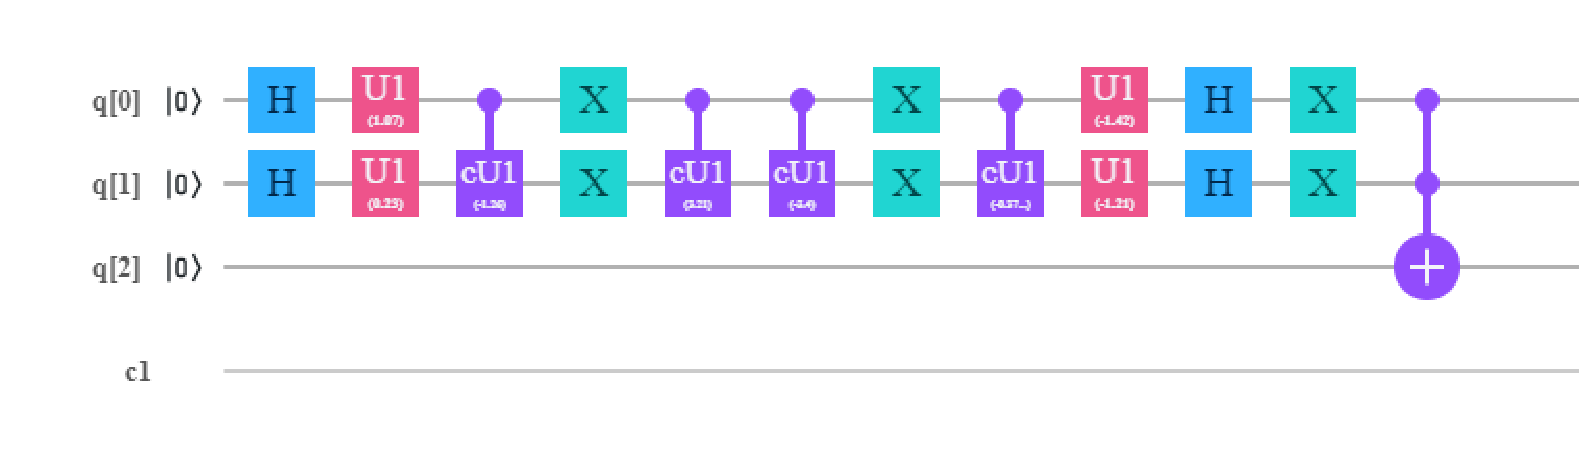
\includegraphics[width=1\textwidth]{img3} \centering \caption{Exemplo de circuito utilizando o algoritmo HSGS.}
\label{TRES} 
\end{figure}


\subsection{Método kernel}

Vamos usar um modelo inspirado nos blocos de rotação de fase, ou seja, vamos construir blocos de variação de módulo. Porém, como precisamos manter a normalização do vetor, vamos sempre alterar em pares, vamos optar por alterar usando o último coeficiente como controle, e vamos nos preocupar com a variação do módulo dos outros coeficientes. Usando a seguinte sequência de operações, podemos variar apenas o primeiro e último coeficiente: $M_{1}=\left(X\otimes\mathbb{I}\right).cX_{0}.cX_{1}.cu_{3}.cX_{1}.cX_{0}.\left(X\otimes\mathbb{I}\right)$, onde $cX_{i}$ in dica que é um $X$ controlado usando o qubit $i$ como de controle e $cu_{3}$ é a versão controlada do operador $u_{3}$, isto é, a rotação de um único qubit com os 3 ângulos de Euler. Esta sequência de operações resulta na seguinte matriz:

\begin{equation}
M_{1}=\left[\begin{array}{cccc}
\cos\left(\frac{a}{2}\right) & 0 & 0 & -\sin\left(\frac{a}{2}\right)\\
0 & 1 & 0 & 0\\
0 & 0 & 1 & 0\\
\sin\left(\frac{a}{2}\right) & 0 & 0 & \cos\left(\frac{a}{2}\right)
\end{array}\right].
\end{equation}
Para o segundo coeficiente podemos usar apenas o operador $cu_{3}.$ Sendo $\theta=\lambda=0$ temos: 
\begin{equation}
M_{2}=\left[\begin{array}{cccc}
1 & 0 & 0 & 0\\
0 & \cos\left(\frac{b}{2}\right) & 0 & -\sin\left(\frac{b}{2}\right)\\
0 & 0 & 1 & 0\\
0 & \sin\left(\frac{b}{2}\right) & 0 & \cos\left(\frac{b}{2}\right)
\end{array}\right].
\end{equation}
E, por fim, para o terceiro coeficiente podemos usar: $M_{3}=cX_{1}.cX_{0}.cX_{1}.cu_{3}.cX_{1}.cX_{0}.cX_{1}$: 
\begin{equation}
M_{3}=\left[\begin{array}{cccc}
1 & 0 & 0 & 0\\
0 & 1 & 0 & 0\\
0 & 0 & \cos\left(\frac{c}{2}\right) & -\sin\left(\frac{c}{2}\right)\\
0 & 0 & \sin\left(\frac{c}{2}\right) & \cos\left(\frac{c}{2}\right)
\end{array}\right].
\end{equation}
Cada uma dessas matrizes altera a amplitude de apenas um dos coeficientes. Quando aplicamos as três, temos na seguinte sequência $U_{a}=M_{3}.M_{2}.M_{1}.$ 
\begin{equation}
U_{a}=\left[\begin{array}{cccc}
\cos\left(\frac{a}{2}\right) & 0 & 0 & -\sin\left(\frac{a}{2}\right)\\
-\sin\left(\frac{a}{2}\right)\sin\left(\frac{b}{2}\right) & \cos\left(\frac{b}{2}\right) & 0 & -\cos\left(\frac{a}{2}\right)\sin\left(\frac{b}{2}\right)\\
-\sin\left(\frac{a}{2}\right)\cos\left(\frac{b}{2}\right)\sin\left(\frac{c}{2}\right) & -\sin\left(\frac{b}{2}\right)\sin\left(\frac{c}{2}\right) & \cos\left(\frac{c}{2}\right) & -\cos\left(\frac{a}{2}\right)\cos\left(\frac{b}{2}\right)\sin\left(\frac{c}{2}\right)\\
\sin\left(\frac{a}{2}\right)\cos\left(\frac{b}{2}\right)\cos\left(\frac{c}{2}\right) & \sin\left(\frac{b}{2}\right)\cos\left(\frac{c}{2}\right) & \sin\left(\frac{c}{2}\right) & \cos\left(\frac{a}{2}\right)\cos\left(\frac{b}{2}\right)\cos\left(\frac{c}{2}\right)
\end{array}\right].\label{matrao}
\end{equation}
Aplicando no estado inicial $\left|\psi_{0}\right\rangle =\left[\begin{array}{cccc}
1 & 0 & 0 & 0\end{array}\right]^{T}$ temos: 
\begin{equation}
\left|a\right\rangle =\left[\begin{array}{c}
\cos\left(\frac{a}{2}\right)\\
-\sin\left(\frac{a}{2}\right)\sin\left(\frac{b}{2}\right)\\
-\sin\left(\frac{a}{2}\right)\cos\left(\frac{b}{2}\right)\sin\left(\frac{c}{2}\right)\\
\sin\left(\frac{a}{2}\right)\cos\left(\frac{b}{2}\right)\cos\left(\frac{c}{2}\right)
\end{array}\right]=\left[\begin{array}{c}
a_{0}\\
a_{1}\\
a_{2}\\
a_{3}
\end{array}\right].
\end{equation}
Então, sabendo os coeficientes $a_{i}$ do vetor $\left|a\right\rangle $, podemos obter os ângulos através das seguintes relações: 
\begin{itemize}
\item $a=2\arccos\left(a_{0}\right)$, 
\item $b=2\arcsin\left(-\frac{a_{1}}{\sin\left(a/2\right)}\right)$, 
\item $c=2\arccos\left(-\frac{a_{2}}{\sin\left(a/2\right)\cos\left(b/2\right)}\right)$. 
\end{itemize}
Se olharmos para a equação (\ref{matrao}), a última linha também já pode ser utilizada como o vetor $\left|b\right\rangle $. Então, se aplicarmos novamente a mesma sequência de operações, mas agora com os seguintes ângulos: 
\begin{itemize}
\item $c=2\arcsin\left(b_{2}\right)$, 
\item $b=2\arcsin\left(\frac{b_{1}}{\cos\left(c/2\right)}\right)$, 
\item $a=2\arcsin\left(\frac{a_{0}}{\cos\left(b/2\right)\cos\left(c/2\right)}\right)$. 
\end{itemize}
Vamos ter: 
\begin{equation}
\left|b\right\rangle =\left[\begin{array}{c}
\sin\left(\frac{a}{2}\right)\cos\left(\frac{b}{2}\right)\cos\left(\frac{c}{2}\right)\\
\sin\left(\frac{b}{2}\right)\cos\left(\frac{c}{2}\right)\\
\sin\left(\frac{c}{2}\right)\\
\cos\left(\frac{a}{2}\right)\cos\left(\frac{b}{2}\right)\cos\left(\frac{c}{2}\right)
\end{array}\right]=\left[\begin{array}{c}
b_{0}\\
b_{1}\\
b_{2}\\
b_{3}
\end{array}\right].
\end{equation}
E aplicando a sequência de operadores $U_{b}\cdot A_{a}$ no estado inicial, tendo que a primeira coluna de $U_{a}$ é $\left|a\right\rangle $ e a última linha de $U_{b}$ é $\left\langle b\right|$: 
\begin{equation}
\begin{split}\left|\psi\right\rangle  & =U_{b}\cdot U_{a}\left|\psi_{0}\right\rangle \\
 & =\left[\begin{array}{cccc}
A_{11} & A_{12} & A_{13} & A_{14}\\
A_{21} & A_{22} & A_{23} & A_{24}\\
A_{32} & A_{32} & A_{33} & A_{34}\\
b_{0} & b_{1} & b_{2} & b_{3}
\end{array}\right]\left[\begin{array}{cccc}
a_{0} & A_{12} & A_{13} & A_{14}\\
a_{1} & A_{22} & A_{23} & A_{24}\\
a_{2} & A_{32} & A_{33} & A_{34}\\
a_{3} & A_{42} & A_{43} & A_{44}
\end{array}\right]\left[\begin{array}{c}
1\\
0\\
0\\
0
\end{array}\right]\\
 & =\left[\begin{array}{cccc}
A_{11} & A_{12} & A_{13} & A_{14}\\
A_{21} & A_{22} & A_{23} & A_{24}\\
A_{32} & A_{32} & A_{33} & A_{34}\\
b_{0} & b_{1} & b_{2} & b_{3}
\end{array}\right]\left[\begin{array}{c}
a_{0}\\
a_{1}\\
a_{2}\\
a_{3}
\end{array}\right].
\end{split}
\end{equation}
Podemos notar que aqui temos $\left|\psi\right\rangle =U_{b}\left|a\right\rangle $. Prosseguindo temos: 
\begin{equation}
\left|\psi\right\rangle =\left[\begin{array}{cccc}
c_{0} & c_{1} & c_{2} & \sum^{3}_{i}a_{i}b_{i}\end{array}\right]^{T}.
\end{equation}
Então o último termo de nosso estado final é $c_{3}=\left\langle b|a\right\rangle $, como queríamos. Lembrando que o valor medido será $\left|c_{3}\right|^{2}=\left|\left\langle b|a\right\rangle \right|^{2}$. Porém, antes de concluirmos precisamos prestar atenção em algumas coisas. Primeiro que a ordem de aplicação dos operadores $M_{i}$ não é independente, e segundo que se olharmos o conjunto de equações que utilizamos para calcular os ângulos $\theta_{i}$ dos operadores $M_{i}$, podemos encontrar alguns problemas. Por exemplo, no conjunto de equações que obtemos para o operador $U_{a}$, temos que $-\sin\left(\frac{a}{2}\right)\sin\left(\frac{b}{2}\right)=a_{1}$ mas se $\left|\sin\left(\frac{a}{2}\right)\right|<a_{1}$ então $\left|\frac{a_{1}}{\sin\left(a/2\right)}\right|>1$ , o que leva à conclusão de que $\sin\left(\frac{b}{2}\right)>1$. Para evitar esse tipo de problema, devemos aplicar diferentes sequências de operações para situações diferentes. Para o vetor $\left|a\right\rangle $ temos simplesmente que para o caso em que $\theta_{i}\leq\theta_{j}\leq\theta_{k}$ vamos aplicar $M_{k}\cdot M_{j}\cdot M_{i}\cdot\left(X\otimes X\right)$. Para o vetor $\left|b\right\rangle $ tendo a mesma sequência $\theta_{i}\leq\theta_{j}\leq\theta_{k}$, de modo análogo aos casos anteriores, utilizamos a ordem inversa, isto é: $M_{i}\cdot M_{j}\cdot M_{k}$, lembrando que os ângulos $a,b,c$ devem ser também recalculados caso a caso.

\section{Resultados numéricos e discussão}

Todos algoritmos foram implementados em Python utilizando a biblioteca NumPy (\url{https://numpy.org/}) para cálculos analíticos e o kit de desenvolvimento Qiskit para Python (\url{https://qiskit.org/}), que fornece não só simuladores quanto acesso a dispositivos reais na nuvem da IBM Quantum Experience (\url{https://quantum-computing.ibm.com/}). Todos os testes em simuladores e a versão quântica do perceptron foi executada a partir do recurso de computação em nuvem disponibilizado pelo Google, chamado Google Colab (\url{https://colab.research.google.com/}). Através desta plataforma o Google disponibiliza um processadores Intel(R) Xeon(R) CPU @ 2.30GHz com 2 núcleos e 12GB de memória RAM. Neste ambiente também foi utilizado a versão 0.16.1 do Qiskit, no qual possui a seguinte versão de seus módulos: 
\begin{itemize}
\item qiskit-aer: 0.7.2, 
\item qiskit-aqua: 0.8.1, 
\item qiskit-ibmq-provider: 0.11.1, 
\item qiskit-ignis: 0.5.1, 
\item qiskit-terra: '0.16.1. 
\end{itemize}
O ambiente disponibilizado pelo Google tem sua conexão encerrada após 12h de duração. Dessa forma para executar a versão quântica dos modelos sigmoide e kernel foi necessário utilizar um computador pessoal para manter a execução por vários dias. Sendo assim, estes modelos foram executados a partir de um computador com processador Intel(R) Core(TM) i5-6400 CPU @ 2.70GHz de 4 núcleos e 8Gb de memória RAM. Por sua vez, neste computador foi utilizada o qiskit versão 0.19.6 com a seguinte versão de seus módulos: 
\begin{itemize}
\item qiskit-terra: 0.14.2, 
\item qiskit-aer: 0.5.2, 
\item qiskit-ignis: 0.3.3, 
\item qiskit-ibmq-provider: 0.7.2, 
\item qiskit-aqua: 0.7.3. 
\end{itemize}

\subsection{Produto interno}

Para comparar o resultado entre os algoritmos propostos (blocos de rotação e HSGS) , foi utilizada a seguinte medida quantitativa de discrepância média proposta por Tacchino e colaboradores \cite{Italiano}:

\begin{equation}
D=\frac{\sum^{n}_{k=1}\left|O^{\left(k\right)}_{IBM}-O^{\left(k\right)}_{ideal}\right|}{n},
\end{equation}
onde para $n$ saídas calculadas, fazemos a diferença entre a saída ideal ($O^{\left(k\right)}_{ideal}$ ), calculada classicamente, e a saída dos dispositivos reais da IBM ($O^{\left(k\right)}_{IBM}$), obtidas através do Qiskit. Devido a limitações impostas no uso do hardware da IBM, como por exemplo filas de utilização, limitamos ao caso com $N=2$ qubits.

Para comparação, primeiro foi reproduzido o modelo binário, onde ao invés de utilizarmos o operador $u_{1}$ responsável por executar uma variação $\theta$ genérica na fase, é utilizado então um operador $Z$ que executa simplesmente uma mudança de sinal. Com $N=2$ qubits, é possível construir $2^{4}=16$ vetores unitários e binários diferentes que geram $n=2^{2^{4}}=256$ produtos distintos possíveis entre si. Foi calculada então a saída esperada analiticamente e a saída obtida através do dispositivo quântico. Neste trabalho, o cálculo foi reproduzido 5 vezes em 3 dispositivos quânticos diferentes, com preferência para o \textit{`ibmq\_vigo'} devido a ter apresentado os melhores resultados. O resultado pode ser visto na Tabela \ref{tabela1}.

\begin{table}[h!]
\caption{Discrepância para o produto interno entre vetores binários}
\label{tabela1} \centering \resizebox{\textwidth}{!}{%
\begin{tabular}{|l|l|l|}
\hline 
\multicolumn{1}{|l|}{\textbf{Dispositivo}} & \textbf{Bloco de rotação}  & \textbf{HSGS} \tabularnewline
\hline 
\multicolumn{1}{|l|}{ibmq\_5\_yorktown} & 0.22016143798828125  & 0.22871780395507812 \tabularnewline
\hline 
\multicolumn{1}{|l|}{ibmq\_valencia} & 0.1013946533203125  & 0.1109771728515625 \tabularnewline
\hline 
\multicolumn{1}{|l|}{ibmq\_vigo} & 0.09790420532226562  & 0.08685302734375 \tabularnewline
\hline 
\multicolumn{1}{|l|}{ibmq\_vigo} & 0.09388351440429688  & 0.08945083618164062 \tabularnewline
\hline 
\multicolumn{1}{|l|}{ibmq\_vigo} & 0.10137939453125  & 0.0917205810546875 \tabularnewline
\hline 
\end{tabular}} 
\end{table}

Podemos notar que não parece haver uma diferença significativa nos resultados. A diferença média entre os resultados dos algoritmos foi de $\left(1.40\pm8.83\right)\times10^{-3}$, isto é, o desvio padrão foi maior que a própria média em módulo. O que indica que podemos esperar que dependendo da execução, um algoritmo ou outro pode se sair um pouco melhor. Este resultado contraria o esperado pelo que consta na literatura. Maior investigação é necessária, mas uma hipótese a ser levantada é que este resultado pode ser decorrente da estrutura dos processadores utilizados. HSGS possibilita uma vantagem significativa em processadores que não possuem operações de múltiplos qubits disponíveis nativamente \cite{Italiano}. Porém como mencionado anteriormente, maior investigação é necessária.

A próxima etapa foi trabalhar com os vetores de valores contínuos. Devido a limitações de tempo e a possibilidade de construção de infinitos vetores contínuos, foi optado por trabalhar com apenas $8$ vetores de valores contínuos gerados aleatoriamente. De maneira que torna-se possível combinar os $8$ vetores para calcularem $n=8^{2}=64$ produtos internos distintos entre si. O resultado é apresentado na Tabela \ref{tabela2}.

\begin{table}[h!]
\caption{Discrepância para o produto interno entre vetores contínuos}
\label{tabela2} \centering \resizebox{\textwidth}{!}{%
\begin{tabular}{|l|l|l|}
\hline 
\multicolumn{1}{|l|}{\textbf{Dispositivo}} & \textbf{Bloco de rotação}  & \textbf{HSGS} \tabularnewline
\hline 
\multicolumn{1}{|l|}{ibmq\_5\_yorktown} & 0.32855645449163706  & 0.338324540019847 \tabularnewline
\hline 
\multicolumn{1}{|l|}{ibmq\_valencia} & 0.1407079724761018  & 0.11474348544855864 \tabularnewline
\hline 
\multicolumn{1}{|l|}{ibmq\_vigo} & 0.10009663220763679  & 0.10272424045323603 \tabularnewline
\hline 
\multicolumn{1}{|l|}{ibmq\_vigo} & 0.11010601938883248  & 0.1821464251602708 \tabularnewline
\hline 
\multicolumn{1}{|l|}{ibmq\_vigo} & 0.1116498082272541  & 0.1082913676285323 \tabularnewline
\hline 
\end{tabular}} 
\end{table}

Seguindo o procedimento adotado para os vetores binários, temos uma média de $\left(-1.10\pm3.27\right)\times10^{-2}$. Como esperado, baseado no resultado dos vetores binários, o desvio padrão é maior que a própria média em módulo e temos o mesmo resultado obtido para o caso binário, isto é, não nos é possível afirmar que nenhum algoritmo é melhor que o outro. A discussão aqui sobre o porque disto ocorrer é a mesma que a anterior, de forma que se torna desnecessário repetir. Além disto, é interessante destacar que a IBM Quantum Experience permite conferir o tempo que cada código levou para ser processado no dispositivo quântico. Neste trabalho pode-se observar que a duração do tempo de processamento de cada código ficou entre 3s e 3.5s geralmente, porém uma análise mais robusta é interessante e possível através dos dados disponibilizados pela IBM.

\subsection{Simulações dos modelos}

Começando com o modelo híbrido de treinamento do perceptron, objetivando reproduzir os resultados que constam na literatura, foi simulado um perceptron binário com 16 entradas (4+1 qubits) utilizando o simulador de computador quântico com ruídos disponível pelo Qiskit através do backend `\textit{qasm\_simulator}'.

O processo decorreu da seguinte maneira: Primeiro foi definido um vetor peso aleatoriamente, e então a partir deste vetor peso foi construído aleatoriamente um conjunto de treinamento consistindo de 50 vetores que resultam em um resultado positivo e 300 que resultam em uma saída negativa. Após gerarmos os dados de treinamento, o vetor peso foi então `esquecido', sendo gerado um vetor peso inicial de maneira aleatória para executarmos o treinamento.

Desta forma, espera-se que durante o treinamento o perceptron seja capaz de recuperar o vetor peso objetivo utilizado na construção do conjunto de treinamentos. Para quantificar este processo de aprendizado, foi utilizada a medida chamada afinidade, que nada mais é que o quadrado do produto interno entre o vetor peso atual e o objetivo, sendo então uma afinidade $1$ quando os dois vetores são idênticos. Também foi utilizada a fração $l=1/2$, isto é, cada vez que a rede classifica errado uma entrada, alteramos o sinal de metade dos componentes do vetor peso, de acordo com a regra de aprendizado discutida em capítulos anteriores.

Também é válido mencionar que a cada novo passo, o algoritmo embaralha a ordem dos dados de treinamento, treinando então em uma nova sequência aleatória. Por fim, com o mesmo conjunto de dados de treinamento, foi treinada a rede 59 vezes reiniciando com um vetor peso inicial definido também aleatoriamente. O treinamento também possui um limite máximo de 3050 passos, isto é, o treinamento é encerrado após o perceptron treinar 3050 vezes utilizando todo o conjunto de dados de treinamento, ainda que não tenha alcançado a afinidade ideal. O resultado encontra-se ilustrado na Figura \ref{img1}.

\begin{figure}[ht]
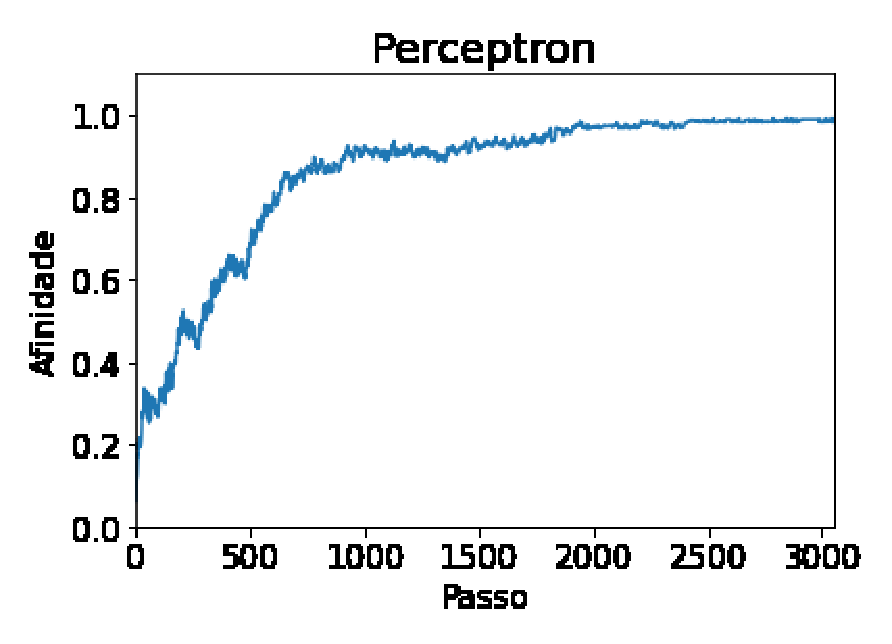
\includegraphics[width=0.5\textwidth]{img1} \centering \caption{Afinidade $\times$ nº de passos no simulador.}
\label{img1} 
\end{figure}

Podemos perceber um comportamento que indica que o perceptron consegue aprender, sendo que o aprendizado ocorre mais rápido nos passos iniciais e se estabiliza em média muito próximo de $1$ por volta dos 2000 passos. Isso sugere que uma tendência de que o neurônio aprenda desde que permita que a rede seja executada uma quantidade suficiente de passos. É interessante notar que devido aos valores binários dos vetores, os valores que a afinidade pode assumir para uma única execução é discretizado, e a proximidade com o valor ideal para uma grande quantidade de passos indica que em uma parcela significativa das execuções o perceptron atingiu o peso objetivo.

Considerando que o sigmoide é um modelo de neurônio naturalmente mais sensível, e com o objetivo de testar a viabilidade deste modelo em computadores quânticos a longo prazo, para simular o sigmoide foi optado então em utilizar o simulador disponibilizado pelo Qiskit chamado `\textit{statevector\_simulator}'. Este simulador, diferente do anterior, não inclui ruídos, ele é um simulador de um circuito quântico ideal.

Observando a função de ativação podemos observar que as entradas (e pesos) aparecem sempre aos pares como argumentos de funções trigonométricas, dessa forma temos na realidade $m-1$ parâmetros livres para $N$ qubits e $m=2^{N}$ estados. O que torna possível representar o mesmo resultado com apenas $m-1$ entradas (e pesos). A partir destas considerações então foi simulado um neurônio com 3 entradas (2+1 qubits).

Seguindo um procedimento análogo ao perceptron, primeiro foi gerado um vetor peso objetivo ideal de 3 componentes definidas aleatoriamente, onde as componentes variam enter $0$ e $2\pi$. Estes valores posteriormente são então codificados como as fases dos coeficientes de amplitude do vetor de estado do sistema.

A partir disto é gerado então um conjunto de treinamento com 200 vetores de entrada definidos aleatoriamente e um peso objetivo também aleatório. A saída ideal é então calculada e, após esta etapa, repetindo o processo adotado para o perceptron, o vetor peso objetivo é `esquecido' e é então gerado um novo vetor peso inicial de maneira aleatória.

Para o treinamento do sigmoide foi adotado um taxa de aprendizagem de $\nu=0.1$ e foram definidas duas condições de paradas: O treinamento deveria se encerrar ou se a função custo fosse reduzida para menos que $10^{-3}$ ou se ela começasse a aumentar. Após aproximadamente 4.000 passos, a função custo reduziu de um valor inicial de aproximadamente $5,75\times10^{-2}$ para aproximadamente $1.74\%$ do seu valor inicial, isto é $1,00\times10^{-3}$. Comportamento este que pode ser conferido na Figura \ref{img2}.

\begin{figure}[ht]
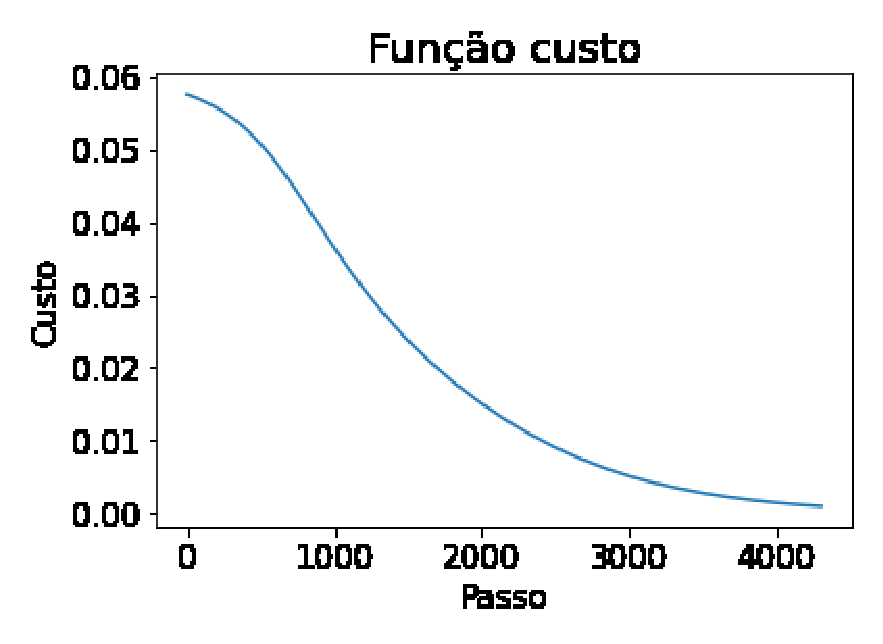
\includegraphics[width=0.5\textwidth]{custo} \centering \caption{Comportamento da função custo para o sigmoide no simulador. }
\label{img2} 
\end{figure}

Como podemos perceber, a função custo sofre um decréscimo conforme era esperado, o que implica que o neurônio sigmoide está aprendendo a partir do conjunto de treinamento. Podemos observar também que com o conjunto de parâmetros que rodamos a rede neural, a função custo aparenta se estabilizar em $1,00\times10^{-3}$, não decrescendo para valores menores que este. Isto está de acordo com o fato de que o encerramento foi feito quando a função custo sofreu um acréscimo. Uma hipótese é que começaria a oscilar em torno deste valor. Caso desejar diminuir ainda mais a função custo, podemos pensar que poderíamos alterar a taxa de aprendizagem, alterar o conjunto de dados de treinamento ou até mesmo utilizar um algoritmo de aprendizado diferente.

Por fim, temos o método kernel. Da mesma forma com o que fizemos no modelo sigmoide, utilizamos o `\textit{statevector\_simulator}'. Para satisfazer as condições discutidas anteriormente, o quadrado centralizado na origem possui um lado de $1.08$, isto é, os pontos podem ser gerados aleatoriamente nas coordenadas $\left(x,y\right)$ sendo $x,y\in\left[-0,54,0.54\right]$. Para o conjunto de treinamento foi gerado uma grade de pontos com espaçamento de $\Delta x=\Delta y=0.04$ entre si e o raio do círculo utilizado para calcular as saídas ideais foi de $0.42$, onde os pontos que estão fora do círculo foram considerados compondo a classe positiva ($+1$) e os pontos no interior compõem a classe negativa ($-1$), novamente, após esta etapa `esquecemos' o raio.

Utilizando estes critérios, então foi calculado um deslocamento $b\approx0.15$. E a partir deste valor de deslocamento, geramos $100$ novos pontos aleatórios no interior do quadrado, destes pontos $99\%$ dos pontos foram classificados corretamente, mais especificamente, $100\%$ dos pontos no interior e $98\%$ dos pontos no exterior foram classificados corretamente. Isso sugere que o círculo que o método kernel aprendeu provavelmente possui um raio ligeiramente maior do que o círculo que utilizamos para gerar nosso conjunto de dados de treinamento. Algumas hipóteses que surgem que poderiam melhorar o resultado é encontrar uma razão entre o lado do quadrado e o raio do círculo com que o método funcione melhor, uma vez que durante este treinamento o raio foi escolhido empiricamente. Ou até mesmo trabalhar com outra superfície ao invés do cone, por exemplo um hiperboloide de uma ou duas folhas.

\subsection{Implementações dos modelos}

Uma vez que o modelo de aprendizado de máquina já tenha sido implementado no simulador utilizando o Qiskit, de maneira geral só precisamos realizar pequenas modificações no código original para executá-lo então em um dispositivo quântico real. Ao invés de enviar o circuito quântico para ser executado em um simulador local disponibilizado pela biblioteca Qiskit, o submetemos para os dispositivos quânticos da IBM via nuvem através da mesma biblioteca, e em sequência obtemos o resultado. Sendo assim, os ajustes não são o maior desafio nesta etapa, porém os dispositivos reais disponíveis para acesso público gratuitamente ainda apresentam muitos desafios. Dentre eles podemos destacar uma quantidade significativa de ruídos, limitações como a quantidade de qubits disponíveis, o tempo extra para submetermos o circuito e recebermos o resultado, e ainda frequentemente nos deparamos com filas de até centenas de códigos esperando para serem executados no mesmo dispositivo, tendo a vista a pouca oferta de opções, aumentando assim significativamente o tempo necessário para executar os treinamentos.

O perceptron é o modelo que mais necessitou adaptações para ser implementado em um dispositivo real. Isto decorre do fato de que para implementarmos o modelo com 16 entradas como feito no simulador, além dos 4 qubits necessários para codificar a entrada e o qubit auxiliar (o que justificava a definição de 4+1 qubit utilizada anteriormente) foi necessário utilizar qubits adicionais para a aplicação do NOT multicontrolado. Porém a IBM Quantum Experience nos fornecesse acesso principalmente a dispositivos com apenas 5 qubits (ou menos), desta forma foi necessário reduzir o número de entradas do peceptron para 4 entradas e implementar um modelo de 2+1 qubit.

A metodologia adotada foi a mesma do simulador, porém com as diferenças de que agora temos 4 entradas, e o conjunto de treinamento é composto por 55 vetores, sendo que 5 resultam em uma saída positiva e 50 uma saída negativa. Além disso reduzimos o limite de passos a cada treinamento para 50 passos e foi executado no dispositivo `\textit{ibmq\_vigo}', que apresentou os melhores resultados dentre os dispositivos quânticos testados anteriormente. O resultado pode ser conferido na Figura \ref{pq}.

\begin{figure}[ht]
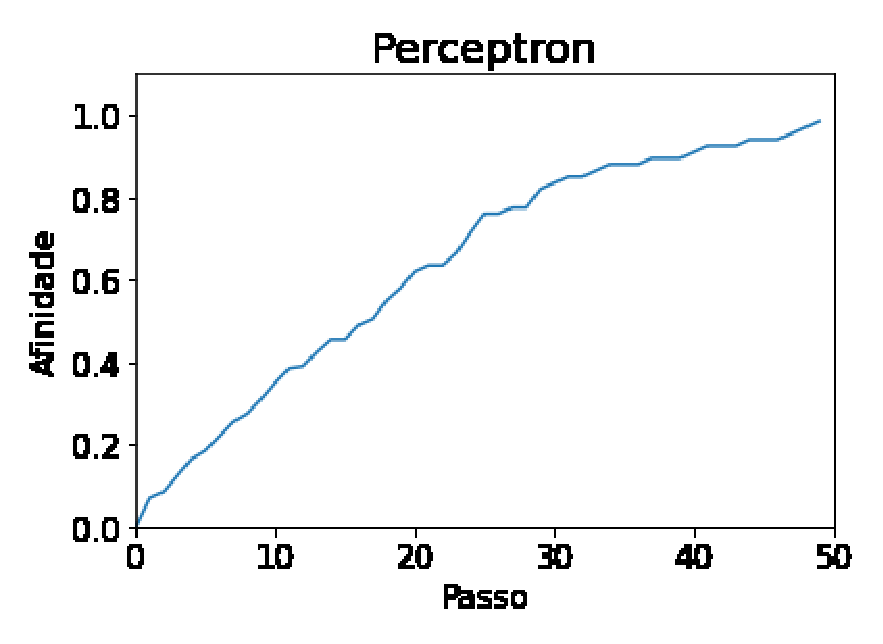
\includegraphics[width=0.5\textwidth]{pq} \centering \caption{Afinidade $\times$ nº de passos no dispositivo quântico.}
\label{pq} 
\end{figure}

Podemos perceber um comportamento similar ao observado no simulador no sentido de que sugere uma tendência de que o perceptron aprenda uma vez que permitimos que ele seja executado por uma quantidade suficiente de passos. Também pode-se notar que ao diminuir pela metade a quantidade de entradas, foi necessário significativamente menos passos para obtermos uma média da afinidade próxima de 1.

Quanto ao sigmoide, considerando que é naturalmente um modelo mais sensível aos ruídos, pensou-se em utilizar um dispositivo quântico que apresentasse um desempenho melhor que os vistos até então, apesar das filas maiores de espera. Para compensar então foi reduzido o conjunto de treinamentos para 50 entradas e foi utilizado o dispositivo `\textit{ibmq\_santiago}'. O volume quântico, abreviado para QV do inglês (\textit{quantum volume}), é uma métrica que a IBM definiu para medir a performance dos seus computadores quânticos reais. Sendo assim, podemos encarar como uma quantificação desta performance, sendo que quanto maior o QV, melhor a performance do dispositvo. Dois dos três dispositivos utilizados até aqui (`\textit{ibmq\_valencia }' e `\textit{ibmq\_vigo }') possuem $QV=16$, enquanto o `\textit{ibmq\_5\_yorktown}' apresenta $QV=8$. A escolha do `\textit{ibmq\_santiago}' se deu por possuir $QV=32$.

Dito isso, foi necessário remover a condição de parada para o treinamento baseado simplesmente no aumento da função custo, uma vez que ela apresentou uma oscilação desde o começo. O resultado pode ser visualizado na Figura \ref{sq}. Paralelamente ao código executado `\textit{ibmq\_santiago}', também foi executado outro idêntico no dispositivo `\textit{ibmq\_5\_yorktown}' ($QV=8$), devido à filas menores, o resultado pode ser conferido na figura \ref{sq2}.

\begin{figure}[ht]
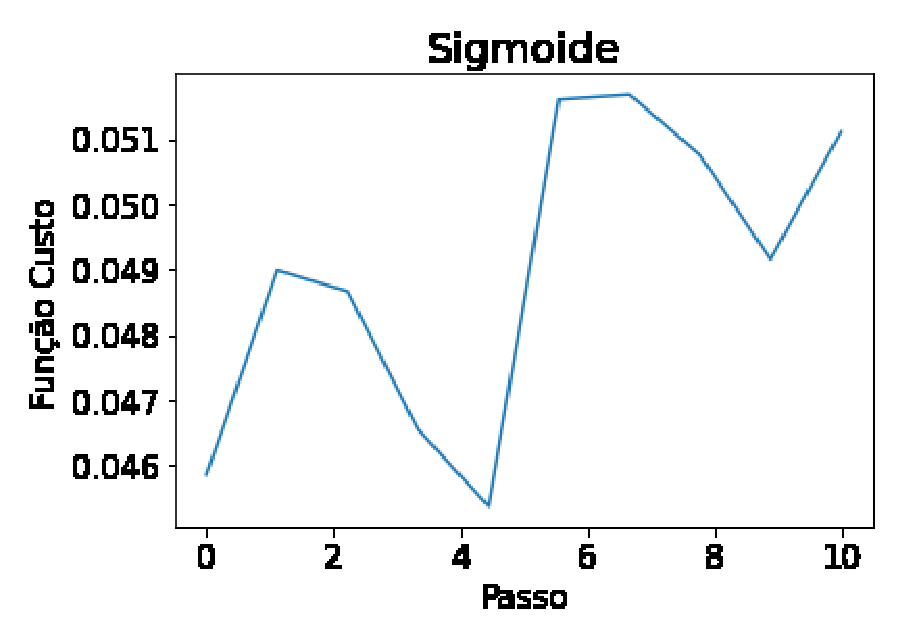
\includegraphics[width=0.5\textwidth]{sq1} \centering \caption{Comportamento da função custo para o sigmoide no dispositivo `\textit{ibmq\_santiago}'. }
\label{sq} 
\end{figure}

\begin{figure}[ht]
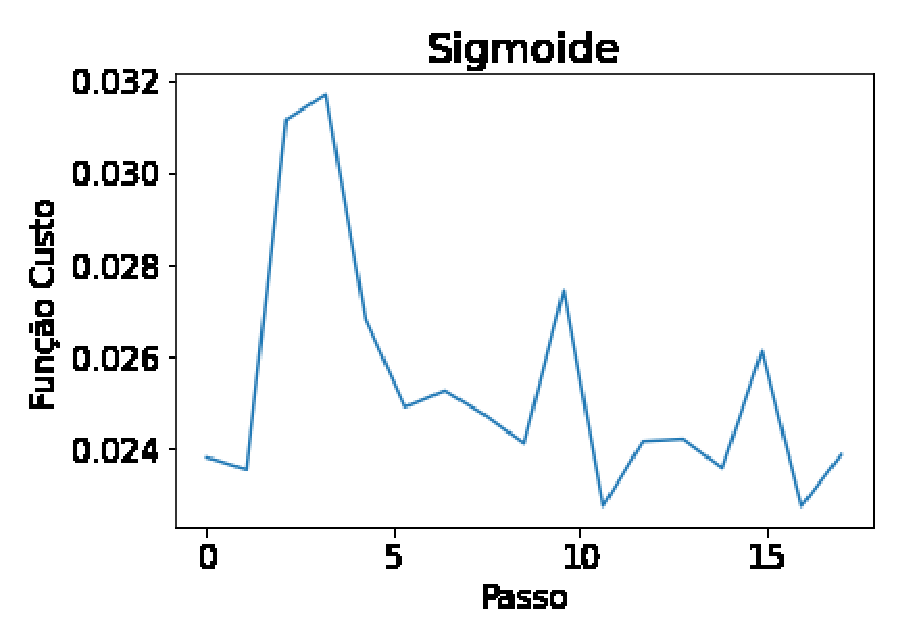
\includegraphics[width=0.5\textwidth]{sq2} \centering \caption{Comportamento da função custo para o sigmoide no dispositivo `\textit{ibmq\_5\_yorktown}'. }
\label{sq2} 
\end{figure}

Graficamente, podemos perceber que há um comportamento oscilatório. E calculando a média dos passos que foram possíveis de serem executados nos dispositivos quânticos reais, 10 no `\textit{ibmq\_santiago}' e 17 no `\textit{ibmq\_5\_yorktown}', temos que o valor custo foram em média $\left(4,90\pm0,23\right)\times10^{-2}$ e $\left(2,54\pm0,25\right)\times10^{-2}$, aproximadamente os mesmos valores iniciais ($4,59\times10^{-2}$ e $2,38\times10^{-2}$). Ou seja, apesar de mostrarmos que o modelo funciona em um dispositivo quântico ideal, ele não aparentou ter capacidade de aprendizagem em um dispositivo quântico real. A hipótese mais provável é que seja devido ao ruído. Para tentarmos melhorar este modelo visando dispositivos atuais ou de curto prazo, poderíamos levantar algumas hipóteses análogas ao discutido sobre como melhorar o modelo implementado no simulador, isto é, alterar a taxa de aprendizagem, o conjunto de dados de treinamento ou até o algoritmo de aprendizado implementado.

Outro ponto é que enquanto o modelo no simulador teve aproximadamente 4.000 passos, no dispositivo quântico tivemos tempo de executar apenas $1$2 devido ao elevado número de cálculos que é necessário serem executados em um dispositivo quântico e as políticas de acesso da IBM aos seus dispositivos públicos. Porém, vale lembrar que em nenhum momento a função custo no simulador aumentou nestes 4.000 passos, enquanto no dispositivo quântico real parece estar flutuando em torno do valor inicial desde o começo, o que é uma característica esperada tendo em vista os problemas de ruídos que os dispositivos atuais ainda enfrentam, uma vez que o modelo sigmoide foi construído para ser sensível a pequenas mudanças. Porém fica em aberto a possibilidade de permitir que o sigmoide rode mais tempo para verificar se em algum momento há alguma tendência de que o neurônio esteja aprendendo, mesmo com os ruídos presentes nos dispositivos atuais.

E por fim temos o método kernel, que diferente dos modelos anteriores não apresenta um processo de aprendizagem gradual que nos permita interromper no meio do processo e obter um resultado parcial para investigarmos alguma tendência de comportamento como fizemos com o sigmoide. Se executado o algoritmo sob as mesmas condições das quais implementamos no simulador, necessitaríamos semanas ou mesmo meses, dependendo das condições, para conseguirmos calcular apenas o deslocamento. Desta forma forma optou-se por diminuir o conjunto de dados de treinamento.

Com esta ideia, foi gerado então uma grade de pontos espaçado $\Delta x=\Delta y=0.08$ entre si dentro do domínio $x,y\in\left[-0,52,0.52\right]$, dessa forma reduziu-se significativamente a quantidade de cálculos necessários. Porém isto aconteceu em troca de precisão, agora utilizando o dispositivo quântico `\textit{ibmq\_vigo }' nosso deslocamento foi de aproximadamente $7,87\times10^{-2}$, aproximadamente $1/2$ do valor obtido no simulador. Além dos desafios habituais de utilizar os dispositivos quânticos reais da IBM, durante o período reservado para a implementação do método kernel, a IBM emitiu um alerta de manutenção, no qual comunicou a aposentadoria de alguns dispositivos quânticos nos próximos dias (incluindo o `\textit{ibmq\_vigo}') e o desligamento temporário de outros, comunicando que isto resultaria em filas de espera ainda maiores para a utilização dos dispositivos durante o período atual.

Então, tendo em vista em vista a limitação de tempo no desenvolvimento do TCC, e a situação que se apresentou, optou-se por executar apenas o treinamento (ou seja, o cálculo do deslocamento) no dispositivo quântico. Esta escolha decorre do fato que uma vez que temos $p$ vetores da classe positiva e $n$ vetores da classe negativa no nosso conjunto do treinamento, o cálculo do deslocamento vai exigir que sejam computados $n^{2}+p^{2}$ produtos internos, enquanto a classificação de um novo ponto necessita da computação de apenas $n+p$ produtos internos. Desta forma, optou-se que o cálculo mais pesado fosse executado no computador quântico.

Utilizando então o circuito implementado no simulador com o peso obtido no dispositivo quântico, classificamos $100$ novos pontos. Destes $54\%$ foram classificados corretamente, porém $100\%$ dos pontos gerados no interior do círculo e aproximadamente $20\%$ dos pontos no exterior. Logo, o raio estimado pelo método consideravelmente maior que o utilizado na fase de geração dos dados de treinamento.

Além da mesma discussão realizada no simulador (como a razão entre os lados do quadrado e o raio do círculo, e a própria superfície em 3 dimensões) este modelo não dá muitas alternativas para melhorar a precisão além de aumentar o conjunto de dados treinamentos ou utilizar um dispositivo com maior precisão. Porém os dispositivos que podem ser utilizados a curto prazo como os dispositivos da IBM apresentam tanto uma quantidade considerável de ruído como filas relativamente longas, exigindo uma grande quantidade de tempo. Fica em aberto a possibilidade de que valia mais apena esperar que um incremento na qualidade dos dispositivo quânticos reais de acesso público, uma vez que já podemos verificar que é um modelo que funciona em um dispositivo ideal.

\section{Conclusão}

Sintetizando então os resultados obtidos durante este trabalho, baseado em um artigo de 2019 \cite{Italiano} foram implementados dois algoritmos para cálculo do produto interno entre vetores binários em um computador quântico. Porém, diferindo dos resultados obtidos na literatura, não foi possível verificar diferença significativa entre os resultados obtidos por cada algoritmo, isto é, as discrepâncias obtida ao calcular o mesmo produto interno no mesmo dispositivo, porém utilizando os dois algoritmos diferentes, não apresentaram diferença significativa entre si. O mesmo pode-se dizer da adaptação que foi proposta e implementada para vetores de valores contínuos. Dentre as hipóteses levantadas para explicar essa discrepância, a principal é a arquitetura dos processadores quânticos.

Quanto aos modelos híbridos de aprendizado de máquina, os três modos foram implementados em simuladores disponibilizados pelo Qiskit, e apresentaram resultados satisfatórios que demonstram um bom potencial quanto à capacidade de aprendizagem de cada modelo. Já sobre a implementação em dispositivos reais, de maneira geral se destaca o problema quanto à demora no processo de submissão do circuito e obtenção de seu resultado, sendo que este problema se sobressaiu quando foi implementado o método kernel, que ainda sofreu o agravante de uma manutenção nos servidores da IBM. Outra dificuldade bastante notável na implementação dos modelos em dispositivos reais são os ruídos, sendo que este problema é notado principalmente durante a implementação do modelo sigmoide, uma vez que foi construído para ser sensível a pequenas variações. Já o perceptron simulado se destaca por ter se mostrado um modelo relativamente robusto quanto aos ruídos e tendo sido capaz de aprender a partir do conjunto de treinamento tanto no simulador quanto no dispositivo real.

Porém vale a pena lembrar que tanto a qualidade do acesso a dispositivos quânticos reais, quanto o problema do ruído nestes dispositivos, são problemas que acredita-se que devem ser mitigados com um maior desenvolvimento tecnológico. Então, uma vez que os modelos se mostram eficientes em um computador idealizado, é coerente supor que venham a ser eficientes em dispositivos reais no futuro. Além disso, outros possíveis caminho para o desenvolvimento futuro deste trabalho é tanto desenvolver os modelos sigmoide e kernel para serem mais tolerantes aos ruídos, quanto desenvolver os modelos para serem mais complexos e/ou eficientes mesmo que ainda em modelos idealizados. Um exemplo que pode-se citar é a implementação de múltiplos qubits em um único computador quântico ou também implementar a etapa de treinamento dos modelos de redes neurais nos computadores quânticos.

Por fim, pode-se destacar que a parte mais desafiadora do trabalho consistiu no estudo e compreensão da modelagem do circuito quântico. Compreender a teoria geral no qual o cálculo dos produtos internos foi construído exigiu conhecimentos de mecânica quântica e computação quântica. Porém uma vez compreendido, permitiu não só implementar o produto interno entre valores binários para o perceptron, como consta na literatura, mas também adaptar para os valores contínuos para os sigmoide e ainda fazer uma adaptação mais extrema para o método kernel. Desta forma, foi demonstrada a viabilidade de uma generalização do perceptron para um modelo de valores contínuos e foi construído um modelo baseado no método kernel que além de ser capaz de efetivamente aprender em dispositivos ideais, serve como uma introdução interessante à área.

Concluindo então, dessa forma acreditamos que o trabalho representa mais um passo no caminho certo do desenvolvimento da inteligência artificial quântica. \bibliographystyle{plain}
\bibliography{referencias}

\end{document}
